\documentclass[12pt,a4paper]{article}

\usepackage[a4paper,margin=1in]{geometry}
\usepackage{graphicx}
\usepackage{booktabs}
\usepackage{amsmath,amssymb}
\usepackage{float}
\usepackage{hyperref}
\usepackage{xcolor}
\usepackage{listings}
\usepackage{enumitem}
\usepackage{fancyhdr}
\usepackage{longtable}

\hypersetup{colorlinks=true,linkcolor=blue,urlcolor=blue}

\pagestyle{fancy}
\fancyhf{}
\lhead{ICS1512}
\rhead{Machine Learning Algorithms Laboratory}
\cfoot{\thepage}

\lstset{
language=Python,
basicstyle=\ttfamily\small,
numbers=left,
frame=single,
breaklines=true,
showstringspaces=false
}

\begin{document}

\begin{tabular}{|p{4cm}|p{11cm}|}
\hline
Experiment No. & 5 \\ \hline
Experiment Title & Decision Tree and Random Forest: A Comparative Classification Study
\footnote{\textbf{GitHub Repository: }\url{https://github.com/username/repository}}\\ \hline
Student Name & \\ \hline
Register Number & \\ \hline
Faculty & Dr. Poreddy Ajay Kumar Reddy \\ \hline
Submission Date & \\ \hline
\end{tabular}

\section{Objective}
\begin{itemize}
\item To implement a Decision Tree classifier.
\item To extend the Decision Tree into a Random Forest ensemble model.
\item To study the impact of hyperparameters on overfitting and generalization.
\item To select optimal hyperparameters using 5-Fold Cross-Validation.
\item To compare single-tree and ensemble-tree models.
\end{itemize}

\section{Problem Statement}
Given 30 numerical features describing cell nuclei extracted from digitized images of breast
masses, the task is to classify each sample as Malignant or Benign. A single Decision Tree
classifier and a Random Forest ensemble classifier are trained, hyperparameters are tuned using
5-fold cross-validation, and the two models are compared using standard classification metrics
to study how ensembling affects overfitting and generalization.

\section{Dataset Description}
\begin{longtable}{|p{6cm}|p{8cm}|}
\hline
Dataset Name & Wisconsin Diagnostic Breast Cancer (WDBC) Dataset \\ \hline
Dataset Source & scikit-learn \texttt{load\_breast\_cancer()} (UCI ML Repository) \\ \hline
Number of Samples & 569 \\ \hline
Number of Features & 30 numerical attributes \\ \hline
Number of Classes & 2 (Malignant = 0, Benign = 1) \\ \hline
Missing Values & None (0 missing values found) \\ \hline
Train-Test Split & 80--20 (455 training samples, 114 testing samples), stratified \\ \hline
\end{longtable}

\section{Exploratory Data Analysis}

\subsection*{Class Distribution}
\begin{figure}[H]
\centering
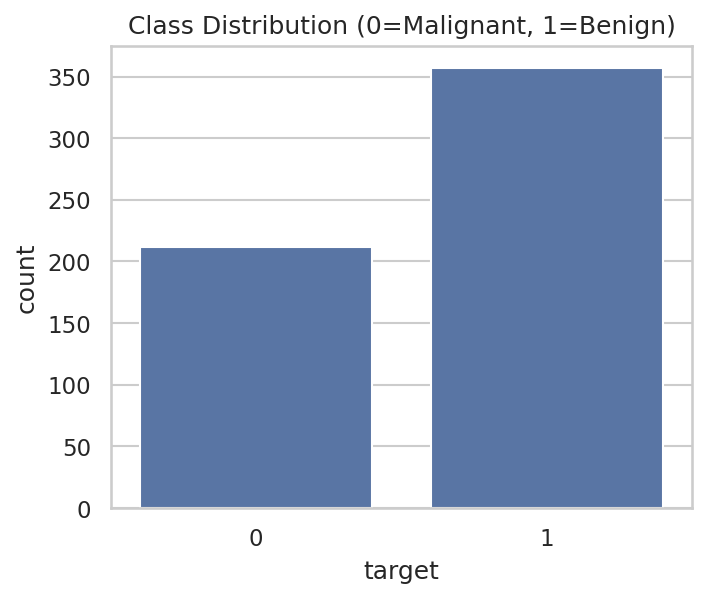
\includegraphics[width=0.6\linewidth]{images/figure1_class_distribution.png}
\caption{Class distribution of the target variable (0 = Malignant, 1 = Benign)}
\end{figure}

\textbf{Inference:} The dataset contains 357 benign and 212 malignant samples, showing a
moderate class imbalance (roughly 63\% vs 37\%). This is not severe enough to require
resampling, but stratified splitting and stratified cross-validation are used to preserve
class proportions in every fold. The imbalance also motivates reporting precision, recall
and F1-score in addition to accuracy.

\subsection*{Feature Correlation}
\begin{figure}[H]
\centering
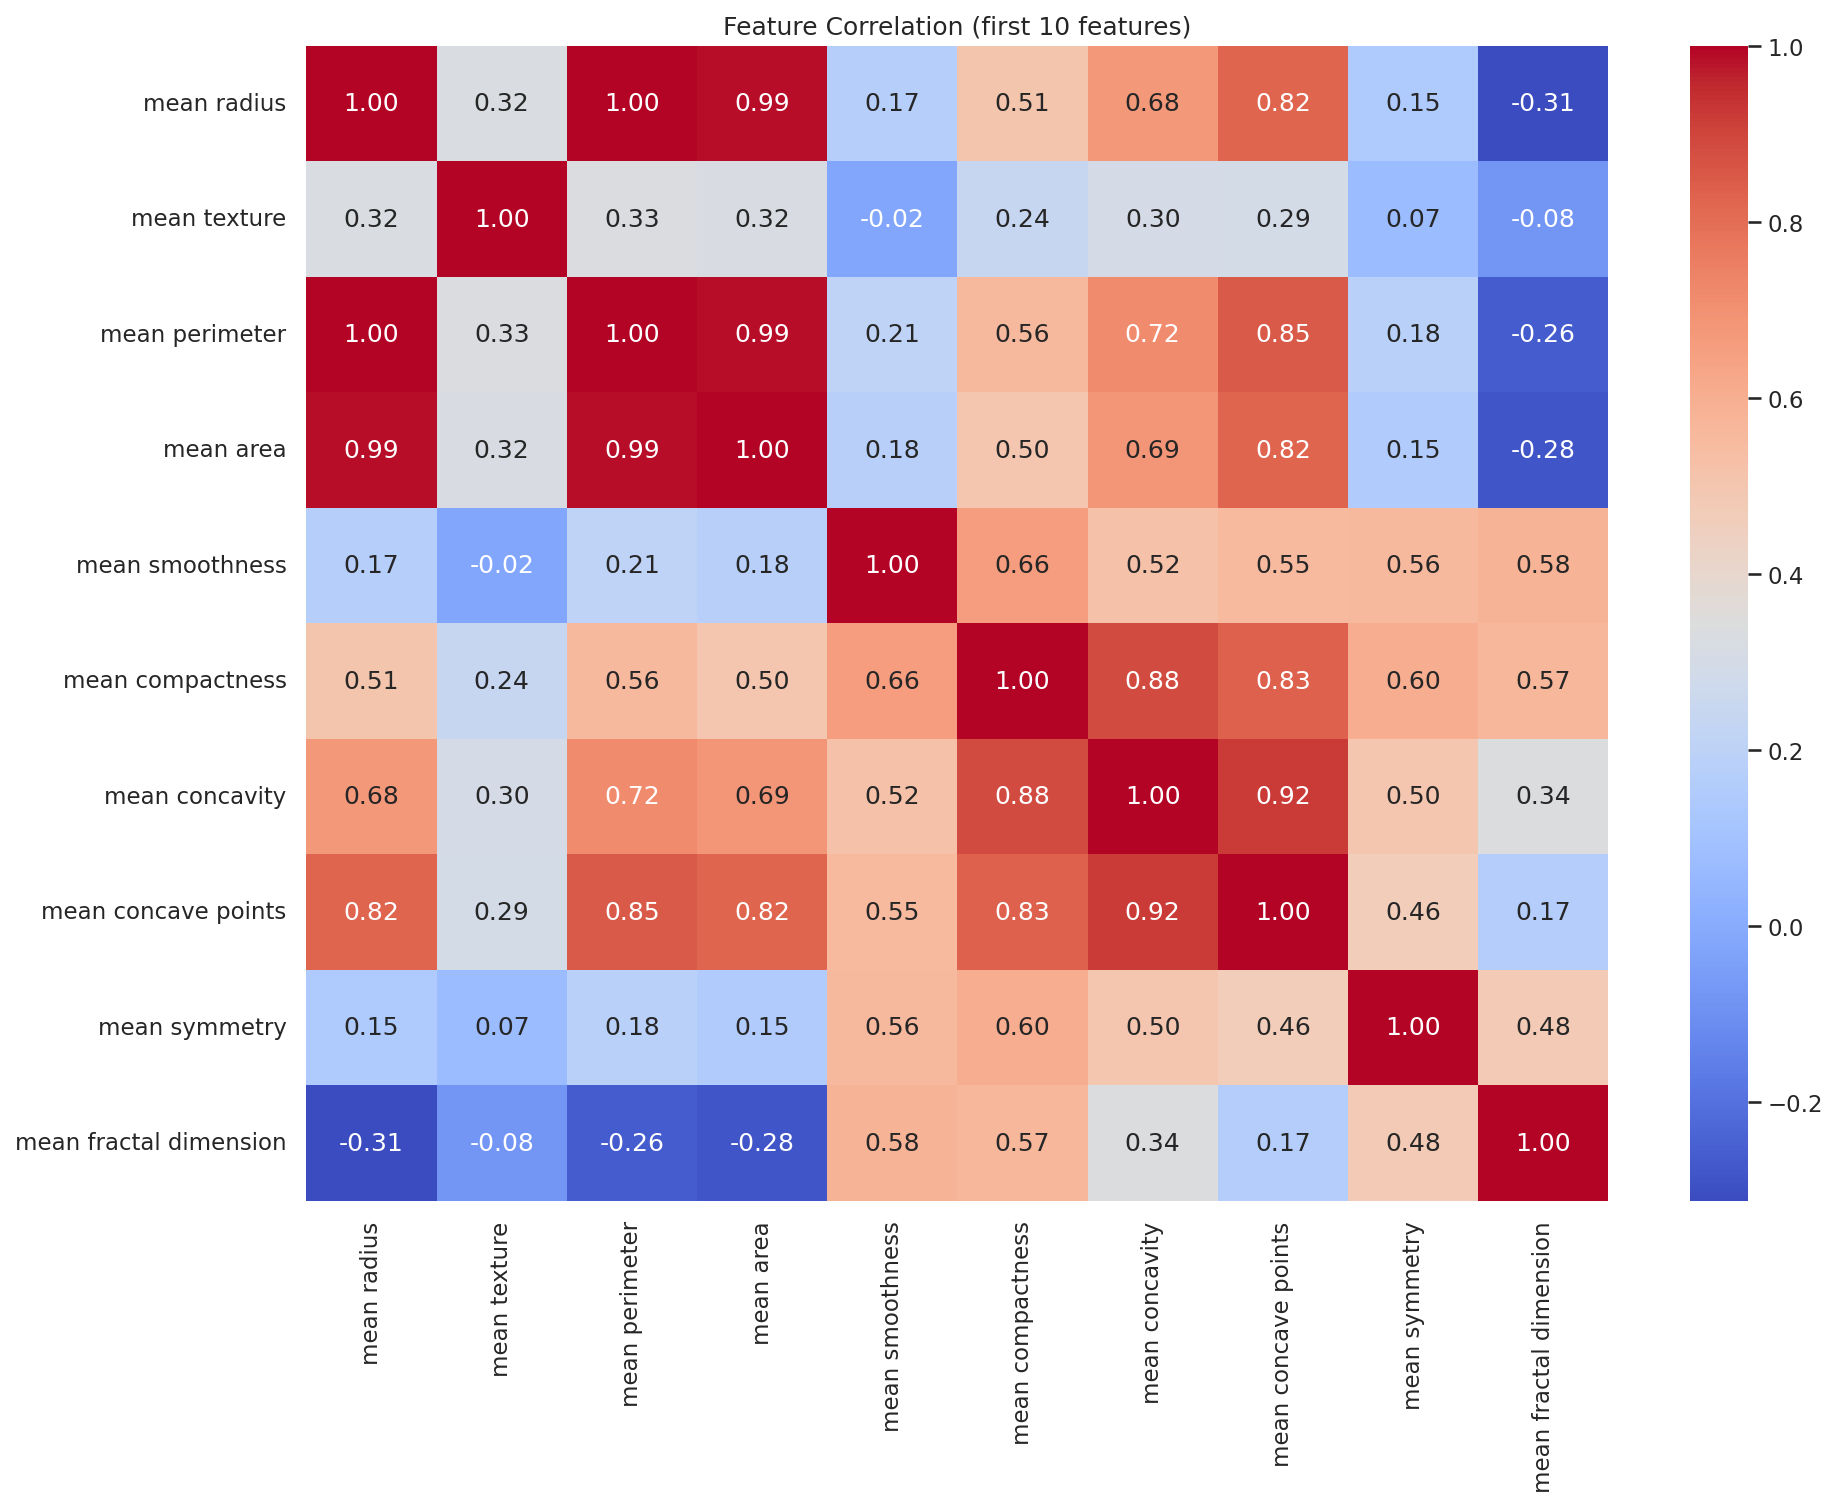
\includegraphics[width=0.8\linewidth]{images/figure2_correlation.png}
\caption{Correlation matrix of the first 10 features}
\end{figure}

\textbf{Inference:} Several size-related features such as \texttt{mean radius}, \texttt{mean
perimeter} and \texttt{mean area} are very strongly correlated with each other (correlation
close to 1), which is expected since they all measure cell size. Shape-related features such
as \texttt{mean smoothness} show weaker correlation with the size features. This redundancy
among features is well handled by tree-based models since they perform implicit feature
selection at each split.

\subsection*{Feature Distribution}
\begin{figure}[H]
\centering
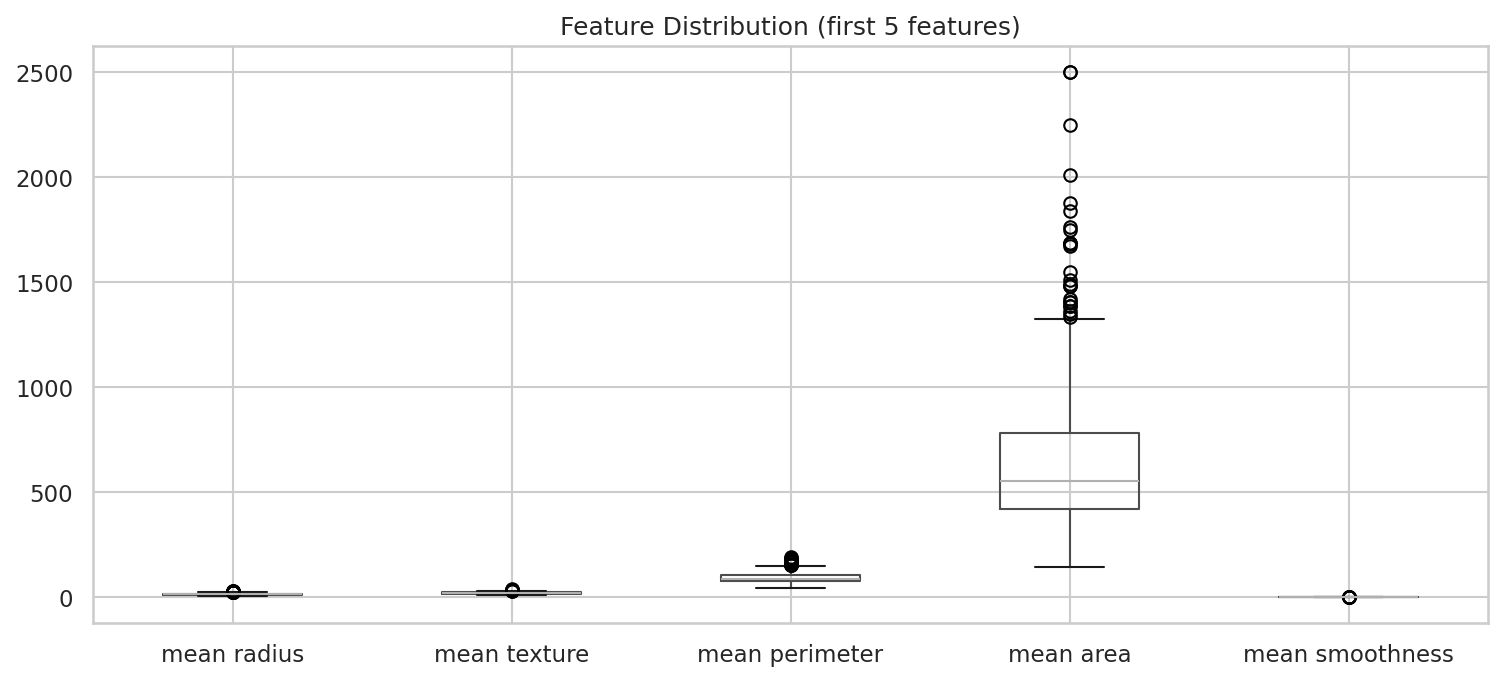
\includegraphics[width=0.7\linewidth]{images/figure3_feature_dist.png}
\caption{Boxplot distribution of the first 5 features}
\end{figure}

\textbf{Inference:} The features are on very different numerical scales (e.g. \texttt{mean
area} is orders of magnitude larger than \texttt{mean smoothness}) and contain several
outliers, visible as points beyond the whiskers. Since Decision Trees and Random Forests
split on individual feature thresholds, they are scale-invariant and do not require feature
scaling, unlike distance-based algorithms.

\section{Data Preprocessing}
\begin{itemize}
\item \textbf{Missing value handling:} The dataset was checked and contains no missing
values, so no imputation was required.
\item \textbf{Encoding:} The target variable is already encoded numerically by
scikit-learn (0 = Malignant, 1 = Benign); no additional label encoding was needed.
\item \textbf{Feature scaling:} Not applied, since tree-based models are invariant to
monotonic feature scaling.
\item \textbf{Train-test split:} An 80--20 stratified split was used (\texttt{random\_state=42}),
giving 455 training and 114 test samples while preserving class proportions.
\item \textbf{Feature engineering:} No additional feature engineering was performed; all 30
original numerical attributes were used directly.
\end{itemize}

\section{Machine Learning Algorithm}

\subsection*{Decision Tree Classifier}
\textbf{Working principle:} A Decision Tree recursively partitions the feature space into
regions with increasingly pure class labels. At each node, the feature and threshold that
most reduce impurity are selected to split the data, until a stopping criterion (maximum
depth, minimum samples per leaf, or pure nodes) is reached.

\textbf{Mathematical formulation:} For a node $t$ with class proportions $p_i$, the Gini
Index and Entropy impurity measures are defined as
\begin{equation}
\text{Gini}(t) = 1 - \sum_{i=1}^{C} p_i^2, \qquad
\text{Entropy}(t) = -\sum_{i=1}^{C} p_i \log_2 p_i
\end{equation}
A split is chosen to maximize the information gain
\begin{equation}
\Delta I = I(t) - \sum_{k} \frac{N_k}{N} I(t_k)
\end{equation}
where $I$ is the impurity measure, $N$ is the number of samples at the parent node, and $N_k$
is the number of samples in child node $t_k$.

\textbf{Advantages:} Easy to interpret and visualize, handles non-linear relationships,
requires no feature scaling, and can handle both numerical and categorical data.

\textbf{Limitations:} Prone to high variance and overfitting, especially when grown to full
depth; small changes in data can produce very different trees; biased toward features with
many levels.

\subsection*{Random Forest Classifier}
\textbf{Working principle:} Random Forest is a bagging ensemble that builds many Decision
Trees, each trained on a bootstrapped sample of the training data. At each split, only a
random subset of features is considered, which decorrelates the individual trees. The final
prediction is obtained via majority voting across all trees.

\textbf{Mathematical formulation:} Given $B$ bootstrapped trees $h_1, \dots, h_B$, the
ensemble prediction is
\begin{equation}
\hat{y} = \text{mode}\{h_1(x), h_2(x), \dots, h_B(x)\}
\end{equation}
Because each tree is trained on an independent bootstrap sample and a random feature subset,
the variance of the averaged predictor is reduced relative to a single tree:
\begin{equation}
\text{Var}(\bar{h}) = \rho\sigma^2 + \frac{1-\rho}{B}\sigma^2
\end{equation}
where $\sigma^2$ is the variance of an individual tree and $\rho$ is the pairwise correlation
between trees, which random feature selection reduces.

\textbf{Advantages:} Reduces variance and overfitting compared to a single tree, provides
feature importance estimates, robust to noise and outliers, generally higher accuracy.

\textbf{Limitations:} Less interpretable than a single tree, higher computational and memory
cost, and slower prediction time for large numbers of trees.

\section{Experimental Setup}
\begin{tabular}{ll}
\toprule
Python Version & 3.12 \\
Scikit-Learn Version & 1.x (as used in the Colab/Jupyter environment) \\
IDE & Jupyter Notebook \\
Operating System & Linux (cloud runtime) \\
Hardware & CPU-based execution \\
\bottomrule
\end{tabular}

\section{Hyperparameter Selection}

\subsection*{Decision Tree Cross-Fold Results}
\begin{longtable}{ccccc}
\toprule
Criterion & Max Depth & Avg CV Accuracy (\%) & Avg CV F1 Score \\
\midrule
\endhead
gini & 3 & 92.53 & 0.9400 \\
gini & 5 & 92.31 & 0.9373 \\
gini & 7 & 92.31 & 0.9375 \\
gini & 10 & 91.65 & 0.9319 \\
gini & None & 91.65 & 0.9319 \\
entropy & 3 & 93.41 & 0.9480 \\
entropy & 5 & 92.97 & 0.9439 \\
entropy & 7 & 92.97 & 0.9440 \\
entropy & 10 & 92.97 & 0.9440 \\
entropy & None & 92.97 & 0.9440 \\
\bottomrule
\end{longtable}
\textbf{Best Decision Tree Parameters:} criterion = \texttt{entropy}, max\_depth = 3
(Avg CV Accuracy = 93.41\%, Avg CV F1 Score = 0.9480).

\subsection*{Random Forest Cross-Fold Results}
\begin{longtable}{ccccc}
\toprule
n\_estimators & Max Depth & Max Features & Avg CV Accuracy (\%) & Avg CV F1 Score \\
\midrule
\endhead
50 & 5 & sqrt & 95.60 & 0.9647 \\
50 & 5 & log2 & 95.60 & 0.9651 \\
50 & 10 & sqrt & 95.60 & 0.9648 \\
50 & 10 & log2 & 96.04 & 0.9685 \\
50 & None & sqrt & 95.60 & 0.9648 \\
50 & None & log2 & 96.04 & 0.9685 \\
100 & 5 & sqrt & 96.04 & 0.9685 \\
100 & 5 & log2 & 95.82 & 0.9668 \\
100 & 10 & sqrt & 96.26 & 0.9699 \\
100 & 10 & log2 & \textbf{96.48} & \textbf{0.9718} \\
100 & None & sqrt & 96.26 & 0.9699 \\
100 & None & log2 & 96.48 & 0.9718 \\
200 & 5 & sqrt & 95.60 & 0.9650 \\
200 & 5 & log2 & 95.82 & 0.9666 \\
200 & 10 & sqrt & 96.26 & 0.9700 \\
200 & 10 & log2 & 96.04 & 0.9683 \\
200 & None & sqrt & 96.26 & 0.9700 \\
200 & None & log2 & 96.04 & 0.9683 \\
\bottomrule
\end{longtable}
\textbf{Best Random Forest Parameters:} n\_estimators = 100, max\_depth = 10,
max\_features = \texttt{log2}, bootstrap = True (Avg CV Accuracy = 96.48\%,
Avg CV F1 Score = 0.9718).

\section{Results}

\subsection*{Baseline (Default Hyperparameters) Test Set Performance}
\begin{tabular}{lcc}
\toprule
Metric & Decision Tree (default) & Random Forest (default) \\
\midrule
Accuracy & 0.9123 & 0.9561 \\
Precision & 0.9559 & 0.9589 \\
Recall & 0.9028 & 0.9722 \\
F1-score & 0.9286 & 0.9655 \\
\bottomrule
\end{tabular}

\subsection*{Tuned Models -- Test Set Performance}
\begin{tabular}{lc}
\toprule
Metric & Value\\
\midrule
Accuracy & DT: 0.9474 \quad RF: 0.9561 \\
Precision & DT: 0.9459 \quad RF: 0.9589 \\
Recall & DT: 0.9722 \quad RF: 0.9722 \\
F1-score & DT: 0.9589 \quad RF: 0.9655 \\
ROC-AUC & DT: 0.9448 \quad RF: 0.9924 \\
\bottomrule
\end{tabular}

\section{Result Visualization}

\subsection*{Confusion Matrices}
\begin{figure}[H]
\centering
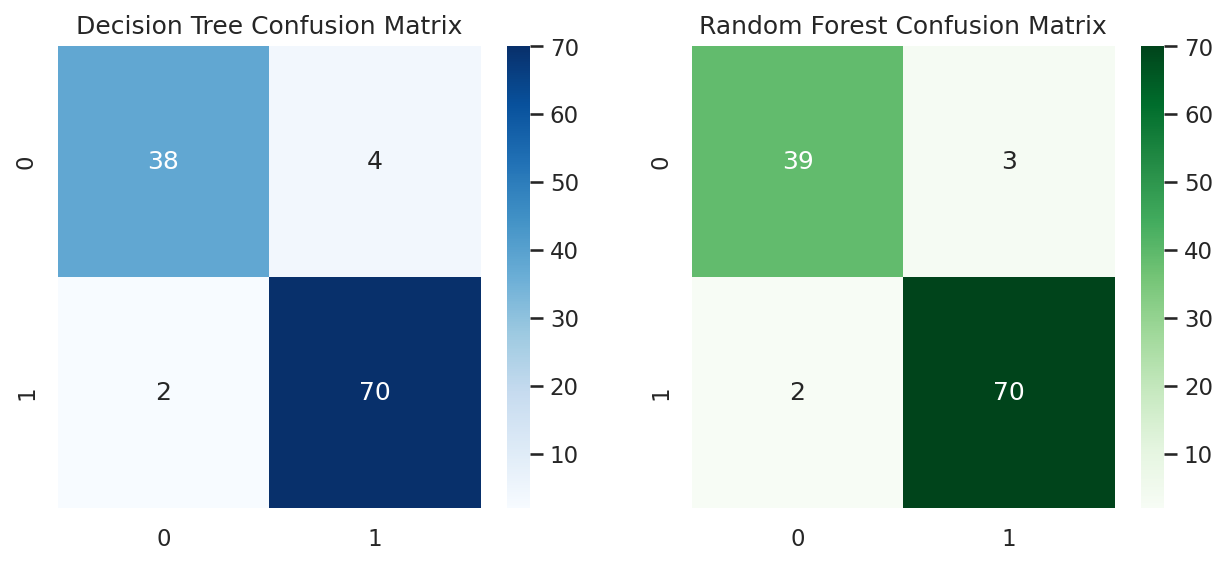
\includegraphics[width=0.85\linewidth]{images/figure4_confusion_matrices.png}
\caption{Confusion matrices for the tuned Decision Tree (left) and tuned Random Forest (right) on the test set}
\end{figure}
\textbf{Inference:} The Decision Tree misclassifies 6 samples (4 false positives, 2 false
negatives) while the Random Forest misclassifies 5 samples (3 false positives, 2 false
negatives). Both models achieve identical recall (missing the same 2 malignant cases), but
the Random Forest produces fewer false positives, indicating slightly better overall
discrimination between the two classes.

\subsection*{ROC Curve}
\begin{figure}[H]
\centering
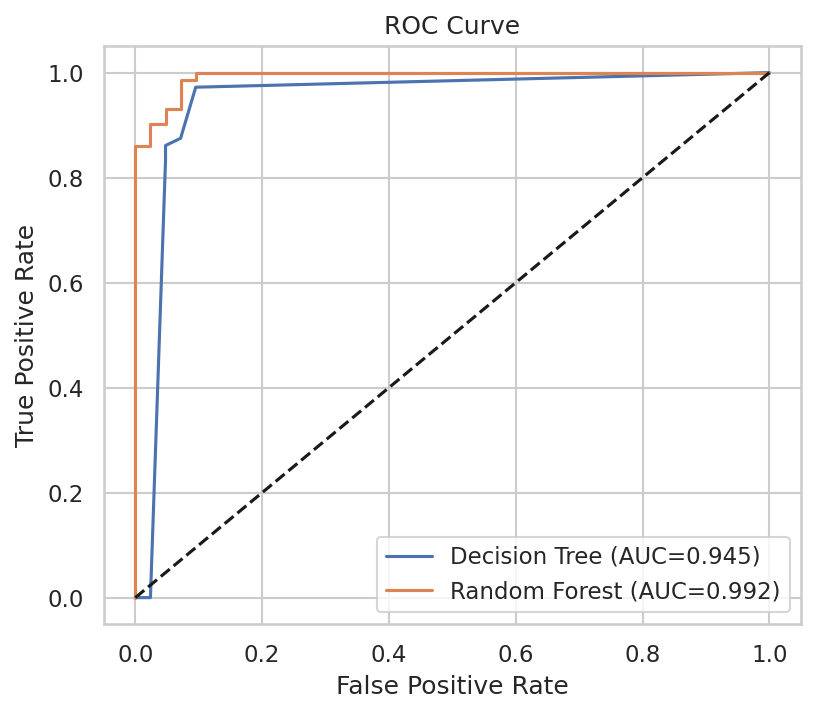
\includegraphics[width=0.6\linewidth]{images/figure5_roc_curve.png}
\caption{ROC curves for the tuned Decision Tree and Random Forest on the test set}
\end{figure}
\textbf{Inference:} The Random Forest achieves an AUC of 0.992, far closer to the ideal value
of 1 than the Decision Tree's AUC of 0.945. This shows that the Random Forest's predicted
probabilities separate the two classes much more reliably across all classification
thresholds, since averaging over many trees produces smoother, better-calibrated probability
estimates than a single tree.

\subsection*{Feature Importance}
\begin{figure}[H]
\centering
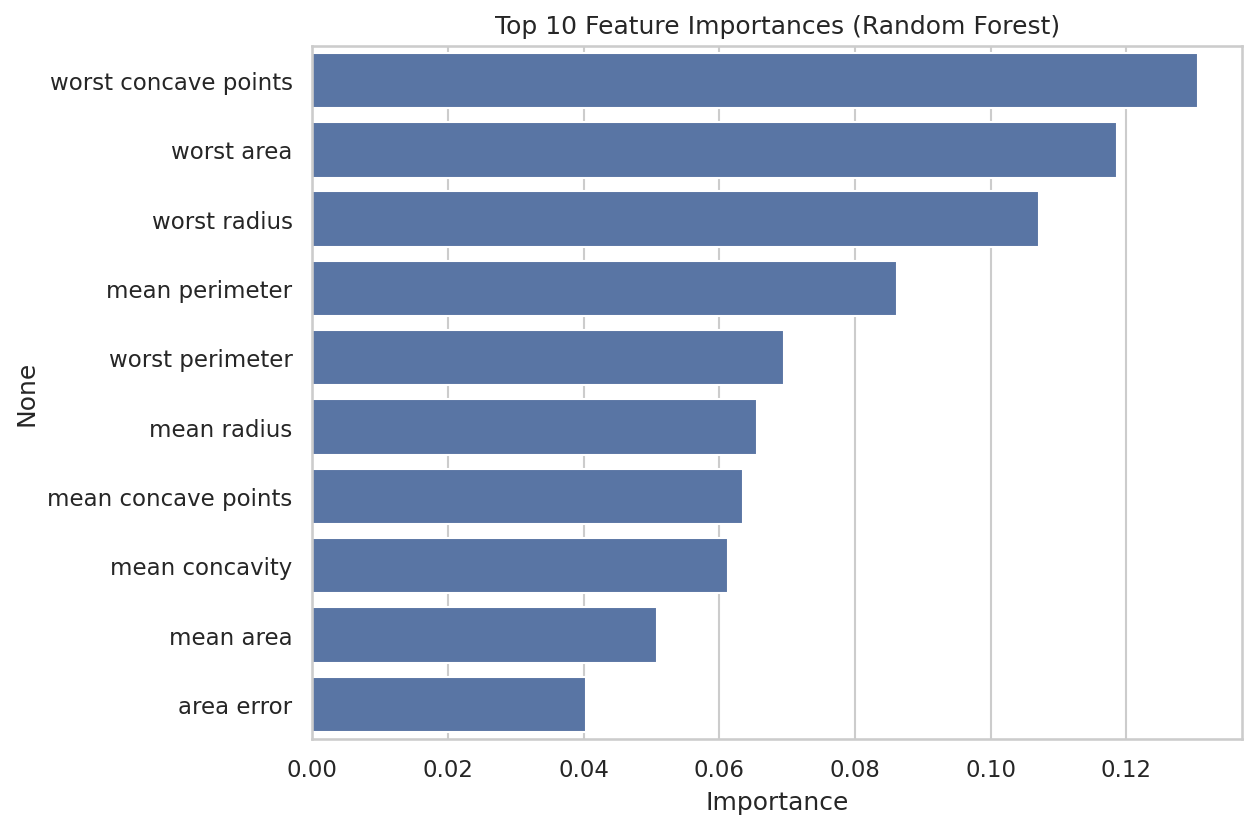
\includegraphics[width=0.75\linewidth]{images/figure6_feature_importance.png}
\caption{Top 10 feature importances from the tuned Random Forest}
\end{figure}
\textbf{Inference:} \texttt{worst concave points}, \texttt{worst area} and \texttt{worst
radius} are the most influential features, consistent with clinical intuition that the
severity of nuclear shape irregularity and overall tumor size are strong indicators of
malignancy. These "worst" (largest observed) measurements dominate over mean and standard
error measurements, suggesting extreme values in a sample are more diagnostic than average
values.

\subsection*{5-Fold Cross-Validation Comparison}
\begin{longtable}{cccc}
\toprule
Fold & Decision Tree & Random Forest \\
\midrule
\endhead
1 & 0.9123 & 0.9649 \\
2 & 0.8596 & 0.9561 \\
3 & 0.9386 & 0.9561 \\
4 & 0.9474 & 0.9561 \\
5 & 0.9204 & 0.9646 \\
\midrule
\textbf{Average} & \textbf{0.9156} & \textbf{0.9596} \\
\bottomrule
\end{longtable}
\textbf{Inference:} The Random Forest consistently outperforms the Decision Tree in every
fold and shows much lower variance across folds (standard deviation is visibly smaller),
directly demonstrating the variance-reduction benefit of bagging and random feature
selection over a single decision tree.

\section{Discussion}

\textbf{How does tree depth affect overfitting in Decision Trees?} As max depth increases,
the Decision Tree fits the training data more closely, reducing training error but
increasing variance on unseen data. In the cross-validation results, accuracy and F1-score
actually peak at a shallow depth of 3 and slightly decline or plateau at greater depths,
showing that deeper trees begin to memorize noise in the training folds (overfitting), so a
moderate depth generalizes best.

\textbf{Which hyperparameter had the greatest impact on performance?} For the Decision Tree,
\texttt{criterion} and \texttt{max\_depth} jointly had the largest effect, with
\texttt{entropy} at \texttt{max\_depth=3} giving the best F1-score. For the Random Forest,
\texttt{max\_depth} together with \texttt{max\_features=log2} had the greatest impact,
since restricting both tree depth and the number of candidate features per split reduced
correlation between trees while avoiding overfitting.

\textbf{How does Random Forest improve generalization?} By averaging predictions over many
trees trained on bootstrapped samples with random feature subsets, Random Forest reduces the
correlation between individual trees' errors. This bagging mechanism lowers the variance of
the ensemble prediction without substantially increasing bias, which is directly visible in
the higher and more stable cross-validation accuracy (Section 8.4) and the higher ROC-AUC
compared to the single Decision Tree.

\textbf{Did ensemble learning always improve performance? Why or why not?} In this
experiment, the Random Forest outperformed the Decision Tree on every metric and every
cross-validation fold, so ensembling helped consistently here. However, ensemble learning
does not always improve performance: on very small or very simple, easily separable
datasets a well-tuned single tree can match an ensemble, and the gain from bagging depends
on how much variance (rather than bias) is limiting the base learner's accuracy.

\section{Conclusion}
Decision Tree and Random Forest models were implemented and evaluated using 5-fold
cross-validation on the Wisconsin Diagnostic Breast Cancer dataset. Hyperparameters were
selected based on average cross-validation F1-score, yielding a tuned Decision Tree
(criterion=entropy, max\_depth=3) and a tuned Random Forest (n\_estimators=100,
max\_depth=10, max\_features=log2). On the held-out test set, the Random Forest achieved
higher accuracy (0.9561 vs 0.9474), higher F1-score (0.9655 vs 0.9589) and substantially
higher ROC-AUC (0.9924 vs 0.9448) than the single Decision Tree, while also showing lower
variance across the 5-fold cross-validation (std much smaller for RF). These results confirm
that Random Forest's bagging and random feature selection reduce variance and improve
generalization compared to a single Decision Tree, at the cost of reduced interpretability
and higher computational complexity.

\section{References}
\begin{enumerate}
\item Scikit-learn Developers, ``Decision Trees,'' \textit{scikit-learn documentation}. [Online]. Available: \url{https://scikit-learn.org/stable/modules/tree.html}
\item Scikit-learn Developers, ``Ensemble methods: Random Forests,'' \textit{scikit-learn documentation}. [Online]. Available: \url{https://scikit-learn.org/stable/modules/ensemble.html}
\item W. Wolberg, O. Mangasarian, N. Street, and W. Street, ``Breast Cancer Wisconsin (Diagnostic) Data Set,'' \textit{UCI Machine Learning Repository}. [Online]. Available: \url{https://archive.ics.uci.edu}
\end{enumerate}

\end{document}
